%================================================================
\section{Method}\label{sec:Method}
%================================================================

%----------------------------------------------------------------
\subsection{Learning the Ising Hamiltonian with Linear Regression}\label{sec:method linreg}
%----------------------------------------------------------------
We want to predict the total energy of the system based on the spin configuration. Assuming no knowledge about the interactions between the spins, a choice of model can be
\begin{equation}\label{eq:general}
    H_{\text{model}}(\mathbf{s}^i) = -\sum_{j=1}^N\sum_{k=1}^N J_{j,k}s_j^is_k^i,
\end{equation}
where $\mathbf{s}^i$ is a particular spin configuration. By collecting all the two-body interactions $\{s_j^is_k^i\}$ for all $i=1,\ldots,N$ in a design matrix $\mathbf{X}$, and all the non-local coupling strengths $J_{j,k}$ in a vector $\mathbf{J}$, we can write this as
\begin{equation*}
    (H_{\text{model}}(\mathbf{s}^1), \ldots, H_{\text{model}}(\mathbf{s}^N))^T = \mathbf{X}\mathbf{J}.
\end{equation*}
With this formulation we can use regression methods from project 1 (OLS, Ridge and Lasso), see \autoref{sec:Appendix A} or \cite{PROJone}, to find the coefficients $\mathbf{J}$.

We generate $N = 10\,000$ spin configurations, each consisting of $40$ spins. The spins take values in $\{-1,1\}$ and are uniformly distributed. The energy of each system is calculated in accordance with \cref{eq:ising 1D energy} for $J=1$.

In order to assess the models, we use the $R^2$ score, given by \autoref{eq:R2}, and mean squared error (MSE), given by \autoref{eq:MSE}, as measures of performance. 

A bias-variance analysis using the bootstrap resampling method for best model selection will also be carried out.

%----------------------------------------------------------------
\subsection{Identifying 2D Ising Model Phases with Logistic Regression}\label{sec:method logreg}
%----------------------------------------------------------------

Here, we use the binary classification method logistic regression, as discussed in \autoref{sec:logreg theory}, to predict if a given state of the two-dimensional Ising model is ordered or disordered. The data, provided by Metha et. al \cite{Mehta_2019}, is a set of spin configurations labeled ordered 1 or disordered 0. The goal is to build a model which will take in a spin configuration and predict whether it constitutes an ordered or disordered phase. The lattices are represented as flattened arrays with $1\,600$ elements instead of a matrix of $40 \times 40$ elements. The dataset is first divided into three pieces, each consisting of either the ordered, disordered or "critical-like" phase. Next, we make training and test sets of the ordered and disordered phases. The remaining critical states will be used as held-out test data which the hope is that we will be able to make good extrapolated predictions on.

\autoref{fig:2d_ising_states} shows some states from the data set for both the ordered and disordered phase, and the critical region as well. 

\begin{figure}[H]
\begin{center}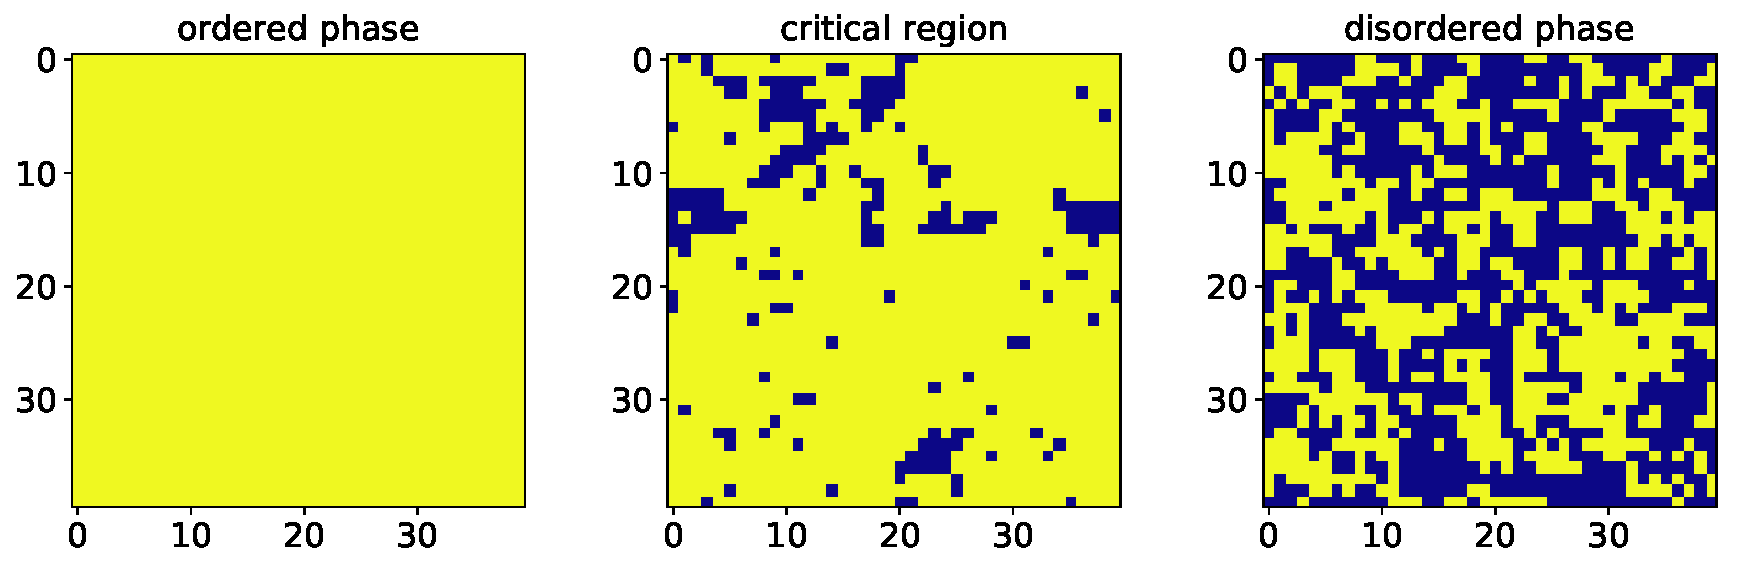
\includegraphics[scale=0.5]{latex/figures/ising_states.pdf}
\end{center}
\caption{figure text}
\label{fig:2d_ising_states}
\end{figure}

GD - find optimal pair values for the learning rate $\eta$ and regularization parameter $\lambda$ the on a small training set by. best pair of values will be which give the highest accuracy score, see \autoref{eq:accuracy score}, for both the training and test set and ultimately the held-out set with the critical states. We will then use the optimal parameters on a larger training set, with the hope that it gives a even higher prediction accuracy.

ROC curve


To conclude the logistic regression analysis, we try to use Newton-Raphson's method for optimization (see \autoref{sec:newton-raphson method}). This method has a notoriously slow iterative scheme, so we will only apply it on a small training set and with few iterations. A ROC curve will also be presented for this method

%----------------------------------------------------------------
\subsection{Neural Networks}\label{sec:method NN}
\subsubsection{Implementation}
For this project, neural networks has been implemented as a python class using standard numpy for linear operations. The architecture can be chosen arbitrarily, i.e. the number of neurons, layers, activation functions and a cost function .

To train the network, one must supply a training set and validation set. The choice of optimization is batch gradient decent. The learning rate, penalty, batch size and number of epoch must be supplied. After each epoch, the accuracy of the network is evaluated and stored using the cost function on both the training data and validation data. This is then used later to evaluate how the network learned.

\subsubsection{Regression on Energy of Generalized Ising Model using Neural 
Networks}

In the same manner as described in \autoref{sec:method datagen}, a set of energies 
as targets were produced by the real Ising model \autoref{eq:ising 1D energy}, but the features were assumed to originate from an unknown model(generalized Ising model). Using a neural network, the energies were attempted learned from the $1600$ features, of which only $80$ have real explanatory ability(those who contribute in the real model). The parameters of the neural network can be summarized in \autoref{tab:nn_params}.


\begin{table}[H]
\caption{Parameters of the neural network.}
\centering
\rowcolors{2}{gray!25}{white}
\begin{tabular}{c|c}
\hline
\hline
Number of Neurons & 400 (one layer)  \\ \hline
Hidden layer activation & $\tanh$   \\ \hline
Output activation & Unmodified  \\ \hline
Cost function & Squared Loss \\ \hline
Learning rate & $7\cdot 10^{-5}$, $9 \cdot 10^{-5}$, $11 \cdot 10{-5}$  \\ \hline
Penalty & $5 \cdot 10{-4}$, $1 \cdot 10^{-3}$, $2 \cdot 10^{-3}$  \\ \hline
Batch size & $100$  \\ \hline
Epochs & $50$  \\ 
\hline
\hline
\end{tabular}
\label{tab:nn_params}
\end{table}

Several models are trained using a grid search using the different learning rates 
and penalties. The R2-score is used to evaluate the models.

To investigate how the networks respond to the dummy features introduced by the generalized Ising model, we introduce a measure "Connection Strength". The connection strength (CS) of a neuron $n^l_j$ is defined as the absolute sum of all the weights that connect that neuron to the next layer:

\begin{equation}\label{eq:CS}
    CS = \sum_i |w^{l+1}_{ji}|
\end{equation}

This is may be though of a measure of how much a particular neuron connects to the next layer. When evaluated on a input feature, we interpret it as how much that feature in particular influence the model. In the case that the CS is zero, the feature has no influence whatsoever.

\subsubsection{Identifying 2D Ising Model Phases with Neural Networks}
The data trained on are the same as described in \autoref{sec:method logreg}, from \cite{Mehta_2019}. The network is trained on the combined orders and disordered states. The model is then evaluated on an independent test set collected from the same combined set. In addition, the model is evaluated on a set consisting of the critical states to explore the generalizability of the model. 

The parameters of the neural network can be summarized in this table:

\begin{table}[H]
\begin{tabular}{|l|l|}
\hline
Number of Neurons & 400, One layer  \\ \hline
Hidden layer activation & Sigmoid   \\ \hline
Output activation & Sigmoid  \\ \hline
Cost function & Cross Entropy \\ \hline
Learning rate & $1e-5$, $2e-5$, $3e-5$  \\ \hline
Penalty & $1e-5$, $1e-4$, $1e-3$  \\ \hline
Batch size & $100$  \\ \hline
Epochs & $50$  \\ \hline
\end{tabular}
\end{table}

Several models are trained using a grid search using the different learning rates 
and penalties. The accuracy score, given by \autoref{eq:accuracy score}, is used to evaluate the models.
%----------------------------------------------------------------